\section{Experimental Results}
The different approaches used for the classification purpose and the corresponding results are described in the following sections. 
\subsection{Approaches and Settings}

\subsubsection*{k-Nearest Neighbor}
The first approach we use is the k-Nearest Neighbor classifier. The parameter k is obtained by performing a parameter search on a leave-one-out cross validation. In terms of accuracy, k equals 16 was the best choice. To weight the different votes, inverse-distance weighting is employed, the distance measure is Manhattan Metric. 

\subsubsection*{Na\"ive Bayes}
Another approach is the Na\"ive Bayes classifier. Despite some attributes obviously not being independent, we still employed this classifier because it proved to be useful in other areas as well.  

\subsubsection*{Decision Tree}
We generated a pruned J48-decision tree. Using sparse parameter search for the confidence factor, we discovered that a tree with 33 nodes delivers the best results in terms of accuracy.

\subsubsection{Neural Network}
A multilayer perceptron is used as a neural network. The structure consists of 15 input neurons (one for each attribute), a hidden layer of five neurons precedes the output layer containing three neurons (one for each class). A learning rate of 0.15 is used, a momentum of 0.075 is applied in each training step. 

\subsection{Results}
To illustrate the accuracy of the different methods employed, the confusion matrices are presented here. All results are found using 10-fold cross validation.

The results of k-Nearest Neighbors are shown in \fref{tab:mat-knn}.

\begin{table}[H]
	\centering
	\caption{Confusion matrix of the k-Nearest Neighbors classifier with Manhattan distance}
	\label{tab:mat-knn}
	\resizebox{\columnwidth}{!}{
	\begin{tabular}[c]{c|ccc||c}
		classified \(\rightarrow\) & \textbf{Low} & \textbf{Medium} & \textbf{High} & Total\\ \hline
		Low & \textcolor{blue}{1167} & 87 & 5 & 1259 \\
		Medium & 203 & \textcolor{blue}{287} & 32 & 522 \\
		High & 23 & 120 & \textcolor{blue}{70} & 213 \\ \hline \hline
		Total & 1393 & 494 & 107 & 1994 \\
	\end{tabular}
}
\end{table}

The results of the Na\"ive Bayes classifier are shown in \fref{tab:mat-nb}.
\begin{table}[H]
	\centering
	\caption{Confusion matrix of the Na\"ive Bayes classifier}
	\label{tab:mat-nb}
	\resizebox{\columnwidth}{!}{
	\begin{tabular}[c]{c|ccc||c}
		classified \(\rightarrow\) & \textbf{Low} & \textbf{Medium} & \textbf{High} & Total\\ \hline
		Low & \textcolor{blue}{1127} & 120 & 12 & 1259 \\
		Medium & 189 & \textcolor{blue}{248} & 85 & 522 \\
		High & 23 & 76 & \textcolor{blue}{114} & 213 \\ \hline \hline
		Total & 1339 & 444 & 181 & 1994 \\
	\end{tabular}
}
\end{table}

The confusion matrix of the decision tree is illustrated in \fref{tab:mat-tree}.
\begin{table}[H]
	\centering
	\caption{Confusion matrix of the decision tree}
	\label{tab:mat-tree}
	\resizebox{\columnwidth}{!}{
	\begin{tabular}[c]{c|ccc||c}
		classified \(\rightarrow\) & \textbf{Low} & \textbf{Medium} & \textbf{High} & Total\\ \hline
		Low & \textcolor{blue}{1141} & 208 & 10 & 1259 \\
		Medium & 200 & \textcolor{blue}{263} & 59 & 522 \\
		High & 30 & 105 & \textcolor{blue}{78} & 213 \\ \hline \hline
		Total & 1371 & 476 & 147 & 1994 \\
	\end{tabular}
}
\end{table}

The results of the neural network classifier can be found in \fref{tab:mat-nn}.
\begin{table}[H]
	\centering
	\caption{Confusion matrix of the Neural Network}
	\label{tab:mat-nn}
	\resizebox{\columnwidth}{!}{
		\begin{tabular}[c]{c|ccc||c}
			classified \(\rightarrow\) & \textbf{Low} & \textbf{Medium} & \textbf{High} & Total\\ \hline
			Low & \textcolor{blue}{1136} & 117 & 6 & 1259 \\
			Medium & 148 & \textcolor{blue}{326} & 48 & 522 \\
			High & 10 & 110 & \textcolor{blue}{93} & 213 \\ \hline \hline
			Total & 1294 & 553 & 147 & 1994 \\
		\end{tabular}
	}
\end{table}

An overview of the different evaluation metrics is presented in \fref{fig:result}.
\begin{figure}[H]
	\centering
	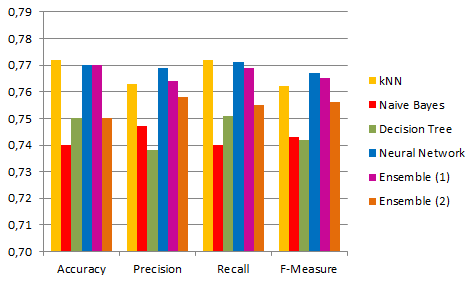
\includegraphics[width=\columnwidth]{../../charts/results.png}
	\caption{Evaluation metrics of the different classifiers}
	\label{fig:result}
\end{figure}

\subsection{Discussion}
Due to the fact that the results do not differ much overall, the efficiency of the different methods is compared. While k-Nearest Neighbors takes the most time by far to reach its conclusion (approximately 30 minutes for a 10-fold cross validation), the Na\"ive Bayes and the decision tree are the fastest classifiers, taking only less than a second. The neural network takes approximately one minute, but delivers the best results. Looking at the confusion matrices, each of the classifiers has its own strength and weaknesses in terms of the different class labels, that can also be seen in \fref{fig:recall}. Based on this observation we look forward to test the majority voting, we hope the results will improve by combining the different approaches. 

\begin{figure}[H]
	\centering
	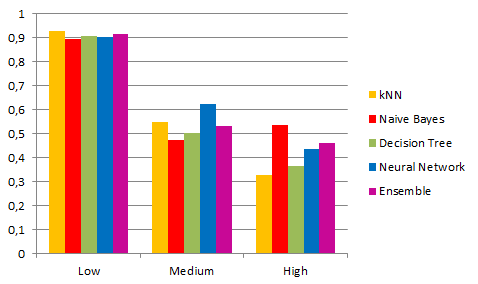
\includegraphics[width=\columnwidth]{../../charts/recall.png}
	\caption{Recall of the different classifiers}
	\label{fig:recall}
\end{figure}

